\chapter{GPU Instruction Listing}

	In this appendix, all instructions of the GPU are listed and explained. On
	the left hand side of each instruction explanation is a diagram showing the
	changes each instruction applies to the stack. Instruction encodings for
	all instructions are shown in figure \ref{encodingfiga}.

	\begin{figure}[H]
		\centering
		\caption{Bit encoding for the different instruction types. All
			instruction types have a fixed width 16-bit encoding.}
		\label{encodingfiga}
		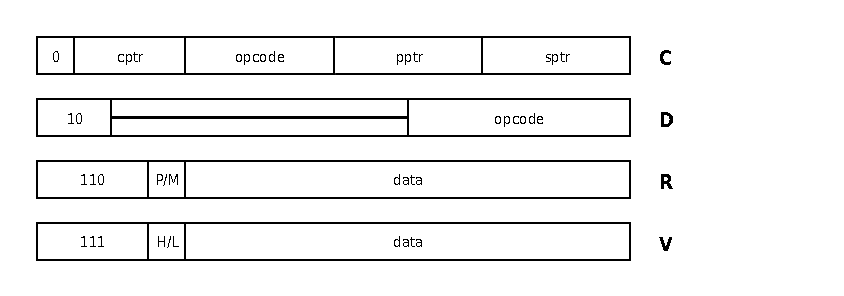
\includegraphics[width=0.75\linewidth]{figure/pdf/instruction_layout} 
	\end{figure}


\newpage

\section{\texttt{C}-type Instructions}
	
	
	\subsection*{\texttt{pushf}}
	
		\begin{wrapfigure}{r}{0.35\textwidth}
			\begin{flushright}
				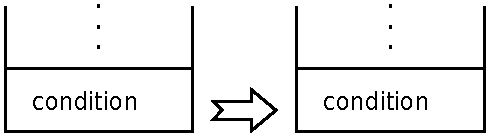
\includegraphics[width=\linewidth]{figure/pdf/i_pushf} 
			\end{flushright}
			\vspace{120pt}
		\end{wrapfigure}
	
			\texttt{cond pushf} sends information from the tread registers to a
			pixel in the frame buffer, if \texttt{cond} is true for the bottom
			value of the stack. Any previous information associated with that
			pixel is overwritten.
			
			Thread register \texttt{1} is used by the frame buffer as a pixel
			id. Pixel ids are sequential, the pixel with the highest id
			corresponds to the lower right corner on the screen, and pixel id
			zero corresponds to the top left pixel.

			Thread register \texttt{2} is used by the frame buffer to determine
			pixel color. The color information must be stored as 24-bit RGB 
			color in the highest 24 bits of the register. The lowest 8 bits of
			register \texttt{2} are not used.
			
			\texttt{pushf} does not affect the stack.
	
	\qquad

	\subsection*{\texttt{pushs}}
	
		\begin{wrapfigure}{r}{0.35\textwidth}
			\begin{flushright}
				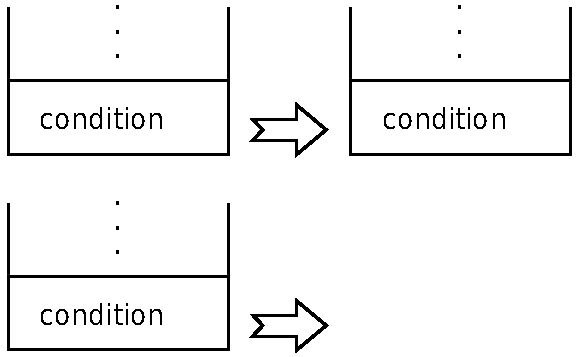
\includegraphics[width=\linewidth]{figure/pdf/i_push} 
			\end{flushright}
			\vspace{80pt}
		\end{wrapfigure}
	
			\texttt{cond pushs} duplicates the current thread and adds it to
			the storage manager with a high execution priority, if
			\texttt{cond} is true for the bottom value of the stack.

			The argument is \emph{not} removed from the stack for the parent 
			thread.

			Thread register \texttt{0} is used to determine where the copied
			thread will start execution when it is sent to a core.

			\texttt{pushs} does not use any of the values on the stack.
			
			No values are returned to the stack of the parent thread.

			\emph{All} values of the stack are discarded for the child thread.
	
	\qquad

	\subsection*{\texttt{pushq}}
	
		\begin{wrapfigure}{r}{0.35\textwidth}
			\begin{flushright}
				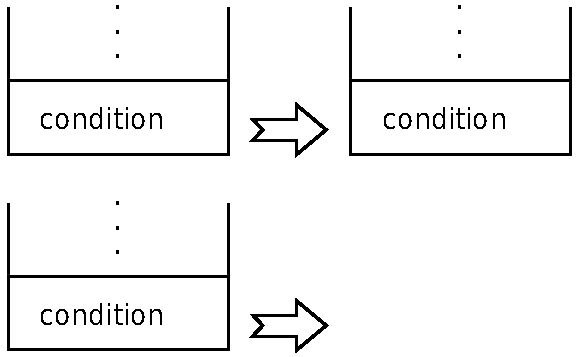
\includegraphics[width=\linewidth]{figure/pdf/i_push} 
			\end{flushright}
		\end{wrapfigure}
	
			\texttt{cond pushq} duplicates the current thread and adds it to the
			storage manager with a low execution priority, if \texttt{cond} is
			true for the bottom value of the stack.

			The argument is \emph{not} removed from the stack for the parent 
			thread.

			Thread register \texttt{0} is used to determine where the copied
			thread will start execution when it is sent to a core.

			\texttt{pushq} does not use any of the values on the stack.
			
			No values are returned to the stack of the parent thread.

			\emph{All} values of the stack are discarded for the child thread.
	
	\qquad

	\subsection*{\texttt{drop}}
	
		\begin{wrapfigure}{r}{0.35\textwidth}
			\begin{flushright}
				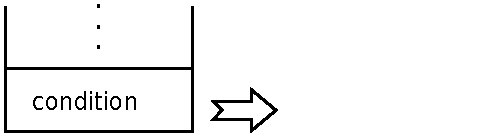
\includegraphics[width=\linewidth]{figure/pdf/i_drop} 
			\end{flushright}
		\end{wrapfigure}
	
			\texttt{cond drop} discards the current thread, if \texttt{cond} is
			true for the bottom value of the stack.
			
			The argument is removed from the stack.
			
			\emph{All} thread registers are discarded.
			
			\emph{All} stack values are discarded.
	
	\qquad

	\subsection*{\texttt{setval}}
	
		\begin{wrapfigure}{r}{0.35\textwidth}
			\begin{flushright}
				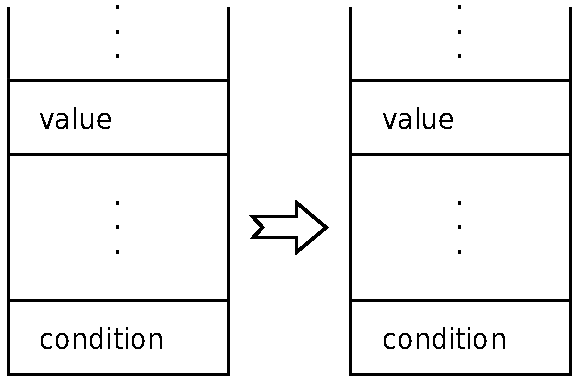
\includegraphics[width=\linewidth]{figure/pdf/i_setval} 
			\end{flushright}
		\end{wrapfigure}
	
			\texttt{cond setval pptr sptr} sets the value of thread register
			\texttt{pptr} to the value on the stack at location \texttt{sptr}, 
			if \texttt{cond} is true for the bottom value of the stack.
			
			The arguments are \emph{not} removed from the stack.
			
			The value of thread register \texttt{pptr} is changed.
			
			No arguments are returned to the stack.
	
	\qquad

\section{\texttt{D}-type Instructions}

	\subsection*{\texttt{abs}}
	
		\begin{wrapfigure}{r}{0.35\textwidth}
			\begin{flushright}
				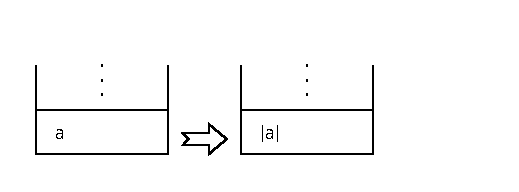
\includegraphics[width=\linewidth]{figure/pdf/i_abs} 
			\end{flushright}
		\end{wrapfigure}
	
			\texttt{abs} computes the absolute value of a fixed-point or
			integer value on the stack.
			
			The argument is removed from the stack.
			
			The result is stored at the bottom of the stack.
	
	\qquad
	
	\subsection*{\texttt{acc}}
	
		\begin{wrapfigure}{r}{0.35\textwidth}
			\begin{flushright}
				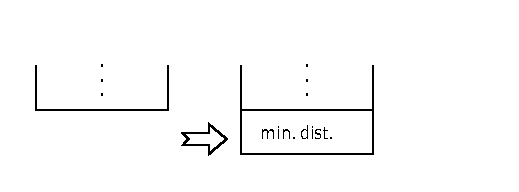
\includegraphics[width=\linewidth]{figure/pdf/i_acc} 
			\end{flushright}
		\end{wrapfigure}
	
			\texttt{acc} returns the accumulated minimum distance updated with
			the \texttt{next} instruction, stored in the core
			
			No arguments are removed from the stack. The accumulated minimum is
			not affected.
			
			The result is stored at the bottom of the stack.
	
	\qquad
	
	\subsection*{\texttt{accid}}
	
		\begin{wrapfigure}{r}{0.35\textwidth}
			\begin{flushright}
				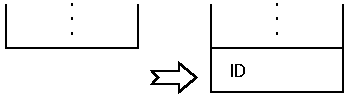
\includegraphics[width=\linewidth]{figure/pdf/i_accid} 
			\end{flushright}
		\end{wrapfigure}
	
			\texttt{accid} returns the ID associated with the accumulated
			minimum distance updated with the \texttt{next} instruction, stored
			in the core
			
			No arguments are removed from the stack. The accumulated minimum is
			not affected.
			
			The result is stored at the bottom of the stack.
	
	\qquad
	
\newpage

	\subsection*{\texttt{add}}
	
		\begin{wrapfigure}{r}{0.35\textwidth}
			\begin{flushright}
				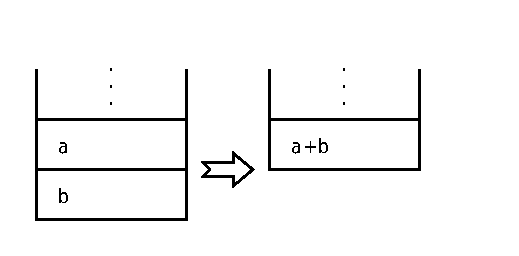
\includegraphics[width=\linewidth]{figure/pdf/i_add} 
			\end{flushright}
		\end{wrapfigure}
	
			\texttt{add} adds two fixed-point or integer values on the stack.
			
			Both arguments are removed from the stack.
			
			The result is stored at the bottom of the stack.
	
	\qquad
	
	\subsection*{\texttt{addv}}
	
		\begin{wrapfigure}{r}{0.35\textwidth}
			\begin{flushright}
				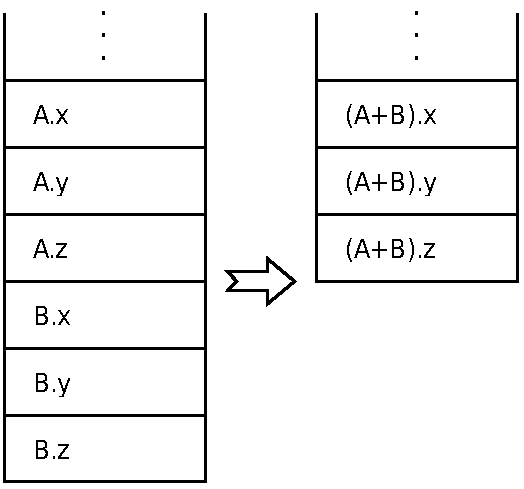
\includegraphics[width=\linewidth]{figure/pdf/i_addv} 
			\end{flushright}
		\end{wrapfigure}
	
			\texttt{addv} adds two three-dimensional fixed-point or integer
			vectors on the stack. Vectors are stored on the stack as three
			consecutive values with the x-coordinate at the top ond the
			z-coordinate at the bottom.
			
			All arguments are removed from the stack.
			
			The result is stored at the bottom of the stack.  \\
			\\
			\\

	
	\subsection*{\texttt{copy}}
	
		\begin{wrapfigure}{r}{0.35\textwidth}
			\begin{flushright}
				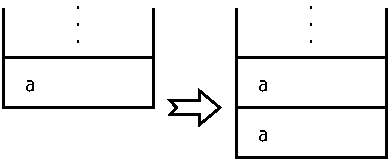
\includegraphics[width=\linewidth]{figure/pdf/i_copy} 
			\end{flushright}
		\end{wrapfigure}
	
			\texttt{copy} duplicates the bottom value of the stack.
			
			The argument is \emph{not} removed from the stack.
			
			The result is stored at the bottom of the stack. \\\\\\
	
\newpage
\section*{}
	
	\subsection*{\texttt{cross}}
	
		\begin{wrapfigure}{r}{0.35\textwidth}
			\begin{flushright}
				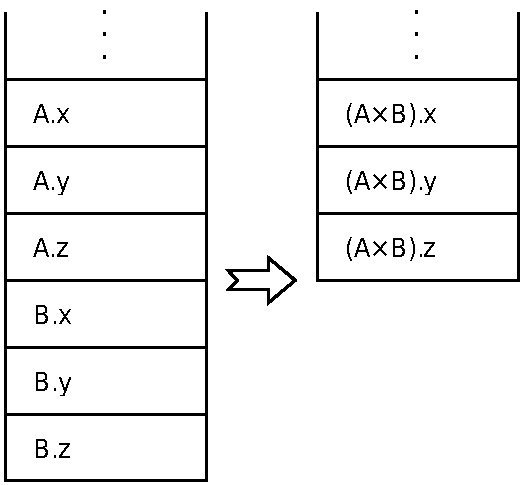
\includegraphics[width=\linewidth]{figure/pdf/i_cross} 
			\end{flushright}
		\end{wrapfigure}
	
			\texttt{cross} computes the cross product of two three-dimensional
			fixed-point or integer vectors on the stack. Vectors are stored on
			the stack as three consecutive values with the x-coordinate at the
			top and the z-coordinate at the bottom.
			
			All arguments are removed from the stack.
			
			The result is stored at the bottom of the stack.\\\\
	
	\qquad\qquad
	
	\subsection*{\texttt{div}}
	
		\begin{wrapfigure}{r}{0.35\textwidth}
			\begin{flushright}
				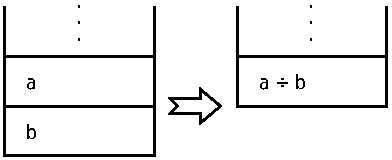
\includegraphics[width=\linewidth]{figure/pdf/i_div} 
			\end{flushright}
		\end{wrapfigure}
	
			\texttt{div} divides two fixed-point or integer values on the
			stack.  The result is undefined if the divisor is zero.
			
			Both arguments are removed from the stack.
			
			The result is stored at the bottom of the stack.
	
	\qquad
	
	\subsection*{\texttt{dot}}
	
		\begin{wrapfigure}{r}{0.35\textwidth}
			\begin{flushright}
				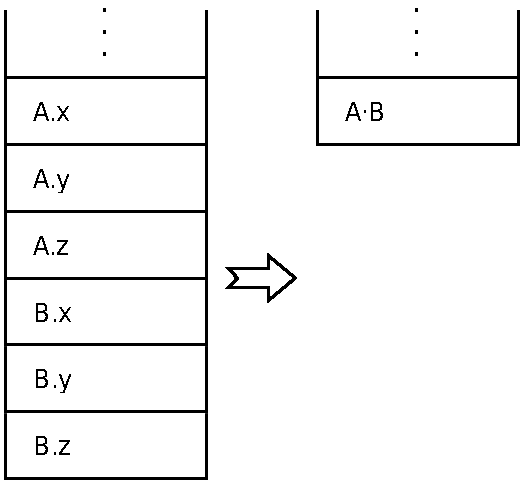
\includegraphics[width=\linewidth]{figure/pdf/i_dot} 
			\end{flushright}
		\end{wrapfigure}
	
			\texttt{dot} computes the dot product of two three-dimensional
			fixed-point or integer vectors on the stack. Vectors are stored on
			the stack as three consecutive values with the x-coordinate at the
			top and the z-coordinate at the bottom
			
			All arguments are removed from the stack.
			
			The result is stored at the bottom of the stack. \\\\\\
	
\newpage
	
	\subsection*{\texttt{dropv}}
	
		\begin{wrapfigure}{r}{0.35\textwidth}
			\begin{flushright}
				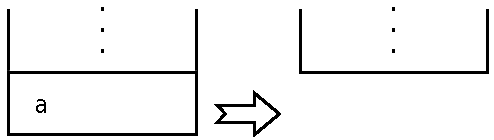
\includegraphics[width=\linewidth]{figure/pdf/i_dropv} 
			\end{flushright}
		\end{wrapfigure}

			\texttt{dropv} removes the bottom argument from the stack.

			The argument is removed from the stack.

			No result.

	\qquad

	\subsection*{\texttt{floor}}
	
		\begin{wrapfigure}{r}{0.35\textwidth}
			\begin{flushright}
				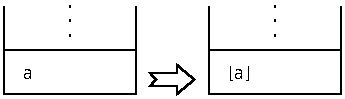
\includegraphics[width=\linewidth]{figure/pdf/i_floor} 
			\end{flushright}
		\end{wrapfigure}
	
			\texttt{floor} rounds a fixed-point value from the stack down to
			the closest whole number. Alternatively, \texttt{floor} rounds an
			integer down to its closest multiple of $2^{16}$.		
	
			The argument is removed from the stack.
			
			The result is stored at the bottom of the stack.
	
	\qquad
	
	\subsection*{\texttt{max}}
	
		\begin{wrapfigure}{r}{0.35\textwidth}
			\begin{flushright}
				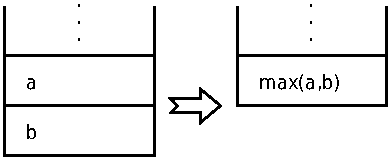
\includegraphics[width=\linewidth]{figure/pdf/i_max} 
			\end{flushright}
		\end{wrapfigure}
	
			\texttt{max} computes the maximum of two fixed-point or integer
			values on the stack. 
	
			Both arguments are removed from the stack. 
	
			The result is stored at the bottom of the stack.
	
	\qquad
	
	\subsection*{\texttt{min}}
	
		\begin{wrapfigure}{r}{0.35\textwidth}
			\begin{flushright}
				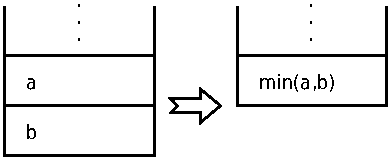
\includegraphics[width=\linewidth]{figure/pdf/i_min} 
			\end{flushright}
		\end{wrapfigure}
	
			\texttt{min} computes the minimum of two fixed-point or integer
			values on the stack. 
	
			Both arguments are removed from the stack. 
	
			The result is stored at the bottom of the stack.
	
	\qquad
	
	\subsection*{\texttt{mul}}
	
		\begin{wrapfigure}{r}{0.35\textwidth}
			\begin{flushright}
				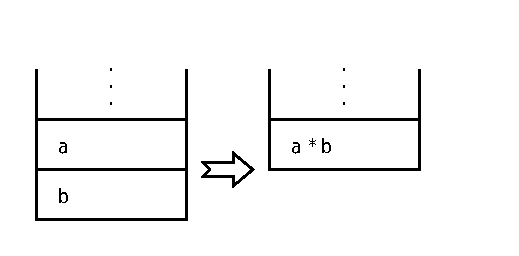
\includegraphics[width=\linewidth]{figure/pdf/i_mul} 
			\end{flushright}
		\end{wrapfigure}
	
			\texttt{mul} multiplies two fixed-point or integer values on the
			stack.
			
			Both arguments are removed from the stack.
			
			The result is stored at the bottom of the stack.
	
	\qquad
	
	\subsection*{\texttt{nop}}
	
		\begin{wrapfigure}{r}{0.35\textwidth}
			\begin{flushright}
				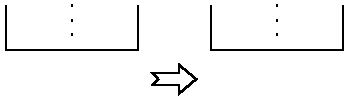
\includegraphics[width=\linewidth]{figure/pdf/i_nop} 
			\end{flushright}
		\end{wrapfigure}
	
			\texttt{nop} does nothing.
			
			No arguments.
			
			No results.
	
	\qquad
	
	\subsection*{\texttt{scale}}
	
		\begin{wrapfigure}{r}{0.35\textwidth}
			\begin{flushright}
				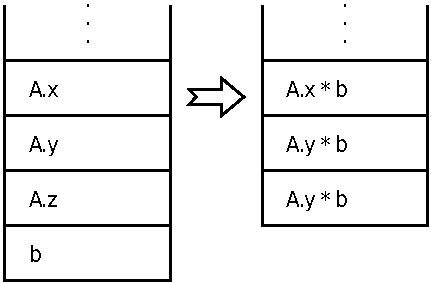
\includegraphics[width=\linewidth]{figure/pdf/i_scale} 
			\end{flushright}
		\end{wrapfigure}
	
			\texttt{scale} multiplies all components of a fixed-point or
			integer vector on the stack with a single scalar factor on the
			stack. Vectors are stored on the stack as three consecutive values
			with the x-coordinate at the top ond the z-coordinate at the
			bottom. The scalar factor must be stored below the vector on the
			stack.
			
			All arguments are removed from the stack.
			
			The result is stored at the bottom of the stack.
	
	\qquad
	
	\subsection*{\texttt{sqrt}}
	
		\begin{wrapfigure}{r}{0.35\textwidth}
			\begin{flushright}
				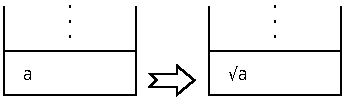
\includegraphics[width=\linewidth]{figure/pdf/i_sqrt} 
			\end{flushright}
		\end{wrapfigure}
	
			\texttt{sqrt} takes the square root an \emph{unsigned} fixed-point
			value on the stack.
			
			The argument is removed from the stack.
			
			The result is stored at the bottom of the stack.
	
	\qquad
	
	\subsection*{\texttt{sub}}
	
		\begin{wrapfigure}{r}{0.35\textwidth}
			\begin{flushright}
				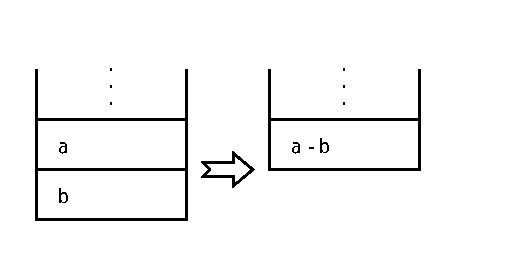
\includegraphics[width=\linewidth]{figure/pdf/i_sub} 
			\end{flushright}
		\end{wrapfigure}
	
			\texttt{sub} subtracts two fixed-point or integer values on the
			stack.
			
			Both arguments are removed from the stack.
			
			The result is stored at the bottom of the stack.
	
	\qquad
	
	\subsection*{\texttt{subv}}
	
		\begin{wrapfigure}{r}{0.35\textwidth}
			\begin{flushright}
				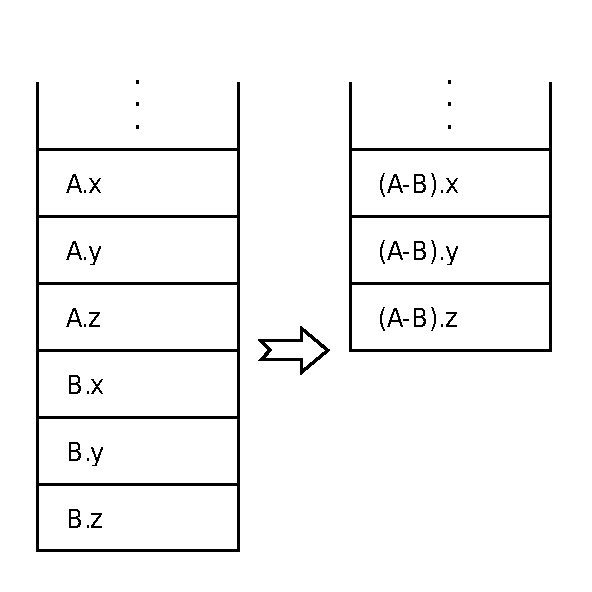
\includegraphics[width=\linewidth]{figure/pdf/i_subv} 
			\end{flushright}
		\end{wrapfigure}
	
			\texttt{subv} subtracts two three-dimensional fixed-point or
			integer vectors on the stack. Vectors are stored on the stack as
			three consecutive values with the x-coordinate at the top ond the
			z-coordinate at the bottom.
			
			All arguments are removed from the stack.
			
			The result is stored at the bottom of the stack.\\\\
	
	\qquad\qquad 
	
	\subsection*{\texttt{swap}}
	
		\begin{wrapfigure}{r}{0.35\textwidth}
			\begin{flushright}
				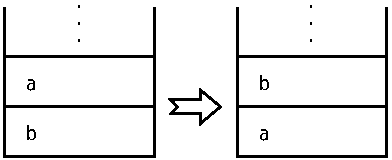
\includegraphics[width=\linewidth]{figure/pdf/i_swap} 
			\end{flushright}
		\end{wrapfigure}
	
			\texttt{swap} swaps two values on the stack.
			
			Both arguments are removed from the stack.
			
			The results are stored at the bottom of the stack.

\newpage
\section{\texttt{R}-type Instructions}

	\subsection*{\texttt{pack}}
	
		\begin{wrapfigure}{r}{0.35\textwidth}
			\begin{flushright}
				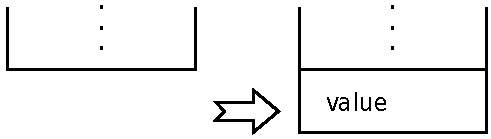
\includegraphics[width=\linewidth]{figure/pdf/i_rtype} 
			\end{flushright}
		\end{wrapfigure}
	
			\texttt{pack pptr} loads the value from thread register 
			\texttt{pptr} to the bottom of the stack.
			
			No arguments are taken from the stack.
			
			The result is stored at the bottom of the stack.
	
	\qquad

	\subsection*{\texttt{val}}
	
		\begin{wrapfigure}{r}{0.35\textwidth}
			\begin{flushright}
				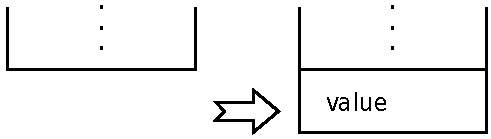
\includegraphics[width=\linewidth]{figure/pdf/i_rtype} 
			\end{flushright}
		\end{wrapfigure}
	
			\texttt{val mptr} loads the value from immutable memory location 
			\texttt{mptr} to the bottom of the stack.
			
			No arguments are taken from the stack.
			
			The result is stored at the bottom of the stack.
	
	\qquad

\newpage
\section{\texttt{V}-type Instructions}

	\subsection*{\texttt{next}}
	
		\begin{wrapfigure}{r}{0.35\textwidth}
			\begin{flushright}
				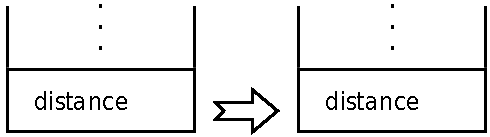
\includegraphics[width=\linewidth]{figure/pdf/i_next} 
			\end{flushright}
		\end{wrapfigure}
	
			\texttt{next id} updates the accumulated minimum distance register
			with the bottom value of the stack as the distance, and \texttt{id}
			as the ID.

			The argument is \emph{not} removed from the stack.
			
			No results are generated on the stack. The accumulated minimum 
			distance register is updated.
	
	\qquad

	\subsection*{\texttt{nextclr}}
	
		\begin{wrapfigure}{r}{0.35\textwidth}
			\begin{flushright}
				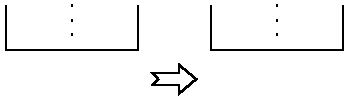
\includegraphics[width=\linewidth]{figure/pdf/i_nop} 
			\end{flushright}
		\end{wrapfigure}
	
			\texttt{nextclr} clears the minimum distance register, setting the
			distance to the largest possible value.

			No arguments are taken from the stack.
			
			No results are generated on the stack. The accumulated minimum 
			distance register is updated.
	
	\qquad
